\author{Kasiński}
\title{Wykład 3}
\documentclass{article}
\usepackage[utf8]{inputenc}
\usepackage{babel}
\usepackage{polski}
\usepackage{float}
\usepackage{graphics}
\maketitle
\begin{document}
	\section{Podejście strukturalne do wyprowadzania modelu stanowego układu złożonego}

		Złożony obiekt sterowania powstaje w wyniku połączenia wielu urządzeń wykonawczych/obróbczych lub
		innych mniejszych obiektów  w sieć przepływu sygnałów charakteryzujących wzajemne
		oddziaływania między tymi urządzeniami.
		Same połączone urządzenia, które na schemacie funkcjonalnym są
		symbolicznie przedstawione jako bloki $U_i$ mogą być same w sobie złożone ze względu na
		dynamikę własną i właściwości statyczne. Wówczas należy je poddać dekompozycji na
		elementarne człony typu SISO połączone wewnętrznie ze sobą.
		
		Za człony elementarne uważać będziemy takie części analizowanego urządzenia, których
		dynamikę można opisać równaniami wejścia-wyjścia niskiego rzędu,
		wyprowadzonymi z klasycznych praw fizyki takich jak: prawa Newtona, prawa Ohma,
		Kirchoffa, prawa Bernouillego. Prawa te odnoszą się do obiektów
		takich, których wymiary liniowe są znacznie mniejsze niż długości fal
		przechodzących przez nie sygnałów. O takich obiektach mówimy, że są obiektami
		o parametrach skupionych.

		W opisie członu elementarnego mogą występować nieliniowości wprowadzane przez
		nieliniową charakterystykę statyczną y = f(x) gdzie y to wartość sygnału na
		wyjściu elementu w stanie ustalonym w odpowiedzi na stałe wymuszenie
		x na jego wejściu.
		Taką nieliniowość może wprowadzać na przykład tranzystor w układzie.
		Innym rodzajem nieliniowości są nieliniowości dynamiczne objawiające się np. występowaniem
		którejś pochodnej sygnału y(t) w innej niż pierwsza potędze po lewej stronie równania
		różniczkowego wiążącego sygnał wyjściowy z sygnałem wejściowym.
		Na przykład
		\begin{equation}
			\dot{y}^2 = x 
		\end{equation}
		Wówczas mamy do
		czynienia z nieliniowym równaniem różniczkowym.
		Praktycznym przykładem takiej nieliniowości niech będą
		sprężyny, które mają nieliniowe charakterystyki jak w przypadku tzw. sprężyn twardych.
		Taki człon musimy traktować jako
		obiekt nieliniowy i oznaczać go jako taki na schemacie blokowym np. podwójną ramką.

		Mamy zatem dwa poziomy dekompozycji opisu złożonego obiektu sterowania: poziom
		wynikający ze schematu funkcjonalnego (podział na urządzenia oraz określenie powiązań
		pomiędzy nimi) oraz poziom podrzędny, wynikający z dekompozycji złożonego urządzenia (na
		podzespoły lub modele otrzymane z dyskretyzacji przestrzennej).
		\subsubsection{Dygresja o elementach o parametrach rozłożonych}
			Rozróżniamy grupę elementów o parametrach rozłożonych takie jak:
			\begin{itemize}
				\item Urządzenia cieplne 
				\item Reaktory chemiczne dużych gabarytów
				\item Długie rurociągi
				\item Długie linie energetyczne
				\item Obwody mikrofalowe
				\item Plastyczne struktury mechaniczne
			\end{itemize}

			Elementy te charakteryzują się dodatkowym etapem analizy dynamicznej
			w sytuacji, gdy nie można jawnie rozwiązać opisujących ich dynamikę równań cząstkowych.
			Tym etapem jest jest dyskretyzacja przestrzenna równań cząstkowych czyli dekompozycja obiektu na układ równań
			zwyczajnych powiązanych poprzez warunki, które są stałe i niezmienne w odpowiednich punktach
			oraz muszą być spełnione, aby uzyskać rozwiązanie. Takie warunki nazywamy warunkami brzegowymi.

			Podsumowując, przy elementach o parametrach rozłożonych konieczna jest dyskretyzacja przestrzenna równań
			cząstkowych. Dyskretyzacja przestrzenna równań cząstkowych to dekompozycja obiektu na układ równań zwyczajnych
			powiązanych przez warunki brzegowe.
	\section{Przykład analizy}
		\begin{figure}
			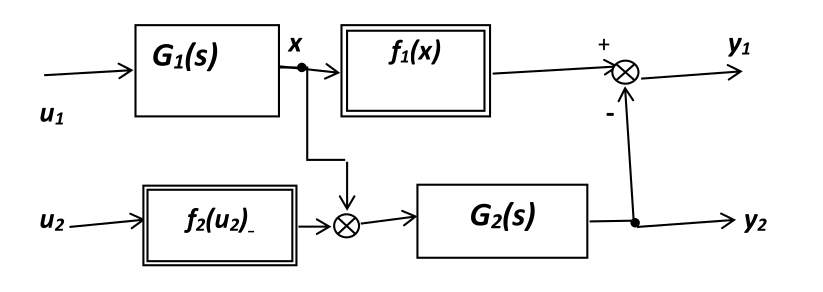
\includegraphics{PrzykladDoAnalizy.png}
		\end{figure}
		Powyższy przykład jest przykładem obiektu MIMO 2x2. 2x2 ponieważ ma dwa sygnały sterujące oraz dwa 
		sygnały kontrolowane nazywane również sygnałami obserwowalnymi. Mamy zatem $ 2 \cdot 2 $ kanałów przepływu
		sygnału do przeanalizowania. 

		$ f_i(.) $ oznaczają charakterystyki statycznych elementów nieliniowych, zakładamy wstępnie,
		że w rozważanych przedziałach wartości ich sygnałów wejściowych są to funkcje
		różnowartościowe, a więc odwracalne; założenie powinno być empirycznie zweryfikowane.

		Bloki dynamiczne są liniowe, a ich dynamika jest reprezentowana przez odpowiednie
		transmitancje operatorowe. Nie ma zatem w ich przypadku problemu z przejściem do
		dziedziny czasu i określenia charakteryzujących te człony równań różniczkowych 
		wejścia-wyjścia.

		Załóżmy, że w przypadku naszych bloków dynamicznych jest spełniony warunek dekompozycji 
		do poziomu prostych elementów dynamicznych. Tak więc będą to równania rzędu co najwyżej
		drugiego rzędu w dodatku liniowe. Do pełnego scharakteryzowania procesów dynamicznych
		realizowanych przez to urządzenie wystarczy znajomość przebiegów sygnałów sterujących
		oraz warunków początkowych dla każdego z równań. Ze spełnienia warunku
		dekompozycji do poziomu elementarnego wynika, że takich warunków jest co najwyżej
		cztery, jeden na każdy kanał.

		Zmienne fazowe określone oddzielnie dla każdego z członów dynamicznych są więc dobrymi
		kandydatami na zmienne stanu całego systemu. Stanowić będą podwektor ogólnego wektora
		stanu, określonego dla całego obiektu. Model stanowy analizowanego obiektu będzie miał
		charakter bloku wektorowo-macierzowego (ze względu na obecność elementów
		nieliniowych):
		\begin{equation}
			\dot{x} = Ax+B[u_1 f_2(u_2)]^T
		\end{equation}

		Warto odnotować w pierwszym równaniu wyjścia obecność tych zmiennych wektora stanu,
		które opisują dynamikę kanału "2 \rightarrow 2". Świadczy to o występowaniu interakcji między
		kanałami głównymi w części wyjściowej urządzenia, co
		ujawnia się na schemacie blokowym. Takie interakcje to są właśnie sprzężenia skrośne
		Co ciekawe, samo równanie stanu części autonomicznej jest liniowe, macierz A nie zawiera żadnych
		nieliniowości. Nieliniowości są obecne w wektorze
		części sterującej i w pierwszym równaniu wyjścia, co odzwierciedla schemat blokowy.

		Wykorzystując odwracalność charakterystyk nieliniowych można w rozważanym przypadku
		sprowadzić nieliniowy model stanowy do wirtualnego modelu liniowego. W tym celu należy
		zdefiniować wirtualny sygnał wejściowy:

		\begin{equation}
			w(t) = f_2^{-1}(u_2)
		\end{equation}

		oraz wirtualny sygnał wyjściowy:

		\begin{equation}
			z(t) = f_1^{-1}(y_1(t))
		\end{equation}

		Wówczas analizowane urządzenie widziane poprzez sygnały $ [ u_1 w ] $ oraz $ [ z y_2 ] $ może być
		postrzegane jako obiekt liniowy. Jeżeli taki zabieg jest możliwy do przeprowadzenia w
		odniesieniu do analizowanego podukładu, to należy z niego skorzystać, gdyż postrzeganie go
		jako obiektu liniowego daje do dyspozycji wiele metod analitycznych opracowanych dla takich
		układów. Jest to lokalna (w sensie: ograniczona do konkretnego urządzenia) linearyzacja
		modelu w dopuszczalna w zakresach zmienności sygnałów w tym układzie,
		w których charakterystyki nieliniowe są odwracalne. Warto jednak pamiętać, że o spełnieniu
		tego warunku decyduje przede wszystkim dynamika układu.

		Nie należy utożsamiać tej metody linearyzacji z linearyzacją punktową nieliniowego układu
		sterowania opisywanego następującymi (ogólnymi) równaniami stanu i wyjścia:

		\begin{equation}
			\dot{x} = f(x, u)
		\end{equation}

		\begin{equation}
			y = h(x)
		\end{equation}

		gdzie pole wektorowe f (tzw. momentum) określa zależność wektora prędkości zmian stanu
		nieliniowego układu dynamicznego od chwilowych wartości zmiennych stanu i sygnałów
		sterujących, czyli jest modelem dynamiki układu.

		\subsubsection{W mądrych słowach, które nie wnoszą nic nowego ale są precyzyjnym opisem}
			Mówimy , że pole f generuje rozmaitość różniczkową stanu układu o wymiarze n,
			odpowiadającą wymiarowi wektora stanu (za wyjątkiem punktów i podrozmaitości zdegenerowanych),
			h jest nieliniową (algebraiczną) funkcją zmiennych stanu (wyjściową), o wymiarze p 
			odpowiadającym liczbie wyjść wielowymiarowego układu nieliniowego O składowych
			funkcji wektorowych f i h zakładamy, że są to funkcje rzeczywiste, analityczne
			(tzn. rozwijalne w szereg Taylora względem swoich argumentów).
	\section{Dygresja na temat poziomu systemowego w układach sterowania w przemyśle)
		\begin{figure}
			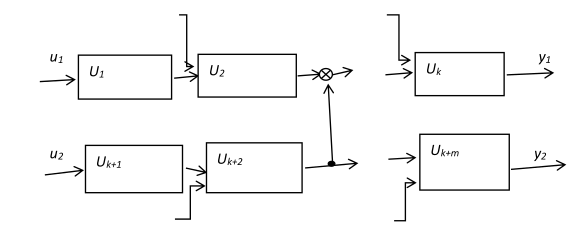
\includegraphics{PoziomSystemowy.png}
		\end{figure}
		Przy produkcji fabrycznej realizowanej w instalacjach przemysłowych, poszczególne
		urządzenia przetwórcze (obiekty sterowania) połączone są ze sobą
		w system
		przetwórczy (system wytwarzania), w sposób wynikający z technologii produkcji lub
		ze zgodnej z logiką procesu produkcyjnego sekwencji przetwarzania materii/energii
		(np. przemian fazowych surowców lub medium nośnego, reakcji chemicznych
		pomiędzy substratami, operacji obróbki półproduktów, itp.).

		W instalacjach przemysłowych mamy do czynienia z przepływami strumieni materii
		(surowców, półproduktów) lub energii, doprowadzanej celem wywołania reakcji
		chemicznej lub przemiany fazowej, albo wyprowadzanej (odprowadzanej) np. w
		przypadku produkcji różnej postaci energii użytkowej lub dla ustabilizowania reakcji
		egzotermicznych, schłodzenia produktów, medium, itp.

		Przepływy mogą mieć charakter szeregowy (kaskadowy, sekwencyjny) np. na linii
		produkcyjnej lub współbieżny (równoległy) w przypadku występowania tzw. węzłów
		(np. w reaktorach wieloskładnikowych, gniazdach obróbczych). Proces może się
		również charakteryzować oddziaływaniami skrośnymi pomiędzy poszczególnymi
		potokami (np. dostarczanie zmodyfikowanego surowca lub półproduktu na linię
		wyrobu, a w szczególności oddziaływaniami zwrotnymi (cofnięcie
		prefabrykatu/produktu/wyrobu do wcześniejszej fazy przetwarzania, celem usunięcia
		wad wykrytych w późniejszej fazie procesu produkcyjnego. Wymienione topologie
		połączeń odzwierciedlone są na schematach blokowych produkcyjnej, na których
		bloki reprezentują poszczególne urządzenia produkcyjne (patrz powyższy rysunek).

		Z punktu widzenia teorii sterowania strumienie masowe i energetyczne uczestniczące
		w procesie są postrzegane poprzez sygnały odzwierciedlające możliwości ich
		modulowania (dawkowania), czyli sygnały wejściowe poszczególnych procesów
		(podprocesów, ogniw łańcucha) oraz sygnały wyjściowe charakteryzujące parametry
		jakościowe produktów (półproduktów) oraz ilościowy wydatek produkcji. Na poziomie
		procesu są to sygnały główne. Oprócz tego występują w modelu dynamiki procesu
		inne sygnały klasyfikowane jako sygnały sterujące (ale nie główne) i inne sygnały
		wyjściowe (również nie główne).

		Urządzenia połączone w system same w sobie mogą być przedmiotem sterowania na
		poziomie lokalnym (operatora urządzenia), albo pracować jako urządzenia
		autonomiczne (sterowane automatycznie, a nawet adaptacyjnie). Mogą także
		podlegać sterowaniu scentralizowanemu na poziomie całego procesu i wówczas ich
		pomocnicze sygnały wejściowe (symbolicznie zaznaczone na schemacie blokowym)
		stają się kolejnymi elementami wektora sterowań procesu, podobnie jak wyjścia
		poszczególnych urządzeń - elementami wektora wyjść procesu. I występują jawnie w
		stanowym modelu ogólnym .całego procesu.
\end{document}
